\chapter{ทบทวนความรู้พื้นฐานเรื่องตรีโกณมิติ}
\section{ตรีโกณมิติเบื้องต้น}
\subsection{องศาและเรเดียน}
\begin{conceptbox}
 \begin{itemize}
    \item[*] เปลี่ยน \textbf{เรเดียน} เป็น \textbf{องศา} แทน $\pi$ ด้วย $180^{\circ}$ 
    \item[*] เปลี่ยน \textbf{องศา} เป็น \textbf{เรเดียน} คูณด้วย $\dfrac{\pi}{180}$
\end{itemize}   
\end{conceptbox}

\begin{examplebox}[NETSAT คณิตศาสตร์ กุมภาพันธ์ 2567]  
$72^{\circ}$ เท่ากับกี่เรเดียน
\begin{enumerate}
\item $\dfrac{2\pi}{3}$
\item $\dfrac{2\pi}{5}$
\item $\dfrac{3\pi}{4}$
\item $\dfrac{3\pi}{5}$
\end{enumerate}
\end{examplebox}

\newpage
\begin{examplebox}[NETSAT คณิตศาสตร์ สิงหาคม 2565]
ถ้า $A$ อยู่ในจตุภาคที่ 1 โดยที่ $0^{\circ}<A<90^{\circ}$ แล้ว $\cos(90^{\circ}-A)$ มีค่าเท่ากับเท่าใด
\begin{enumerate}
\item $\sin(A)$
\item $\cos(A)$
\item $-\sin(A)$
\item $-\cos(A)$
\end{enumerate}
\end{examplebox}

\begin{examplebox}[NETSAT คณิตศาสตร์ สิงหาคม 2565]
กำหนด $0^{\circ}<A<90^{\circ}$ แล้วจงหาค่าของ 
\[\sin(90^{\circ}-A)\cos(A)\tan^2(A)+\dfrac{\sin(A) \cos(90^{\circ}-A)}{\tan^2(A)}\]
\begin{enumerate}
\item $-1$
\item $1$
\item $\sin(2A)$
\item $\cos(2A)$
\end{enumerate}
\end{examplebox}

\begin{examplebox}[NETSAT คณิตศาสตร์ กุมภาพันธ์ 2565]
ถ้า $\tan(\theta)=-10$ เมื่อ $90^{\circ}<\theta<180^{\circ}$ แล้ว $\cos(\theta)$ มีค่าเท่าไร
\begin{enumerate}
\item $\dfrac{-1}{\sqrt{101}}$
\item $\dfrac{1}{\sqrt{101}}$
\item $\dfrac{10}{\sqrt{101}}$
\item $\dfrac{-10}{\sqrt{101}}$
\end{enumerate}
\end{examplebox}

\begin{examplebox}[NETSAT คณิตศาสตร์ กุมภาพันธ์ 2565]
ถ้า $\theta$ เป็นมุม ซึ่ง $270^{\circ}<\theta<360^{\circ}$ และ $\sin(\theta)=-\dfrac{1}{4}$ แล้ว $\sin(2\theta)$ มีค่าเท่าไหร่
\begin{enumerate}
\item $-\dfrac{\sqrt{15}}{8}$
\item $\dfrac{\sqrt{15}}{8}$
\item $-\dfrac{\sqrt{15}}{4}$
\item $\dfrac{\sqrt{15}}{4}$
\end{enumerate}
\end{examplebox}

\begin{examplebox}[NETSAT คณิตศาสตร์ สิงหาคม 2565]
ถ้า $\tan(\theta)=3$ สำหรับ $0^{\circ}<\theta<90^{\circ}$ แล้ว $\cos(\theta)+\sin( \theta)$ มีค่าเท่าไร
\begin{enumerate}
\item $\dfrac{1}{\sqrt{10}}$
\item $\dfrac{2}{\sqrt{10}}$
\item $\dfrac{3}{\sqrt{10}}$
\item $\dfrac{4}{\sqrt{10}}$
\end{enumerate}
\end{examplebox}

\begin{examplebox}[NETSAT คณิตศาสตร์ สิงหาคม 2566]
กำหนดให้ $\tan(\theta)=3$ เมื่อ $0^{\circ}<\theta<90^{\circ}$ และ $x=\cos(\theta), y=\sin(\theta)$ ข้อใดถูกต้อง
\begin{enumerate}
\item $x y=\dfrac{3 \sqrt{10}}{5}$
\item  $x-y=\dfrac{\sqrt{10}}{5}$
\item  $x+y=\dfrac{2 \sqrt{10}}{5}$
\item  ถูกต้องข้อ 1, 2 และ 3
\end{enumerate}
\end{examplebox}

\newpage
\section{กฏของกฎของไซน์และโคไซน์}
\begin{theorembox}[กฏของโคไซน์]
กำหนดให้ $\triangle ABC$ มีความยาวแต่ละด้านซึ่งแสดงดังรูปที่~\ref{Figure25} เราจะได้ความสัมพันธ์ว่า
\begin{align*}
a^2&=  b^2+c^2-2bc\cos(A)\\
b^2&=  c^2+a^2-2ca\cos(B)\\
c^2&=  a^2+b^2-2ab\cos(C)\\
\end{align*}
\end{theorembox}
 \begin{figure}[H]	 
	\centering
	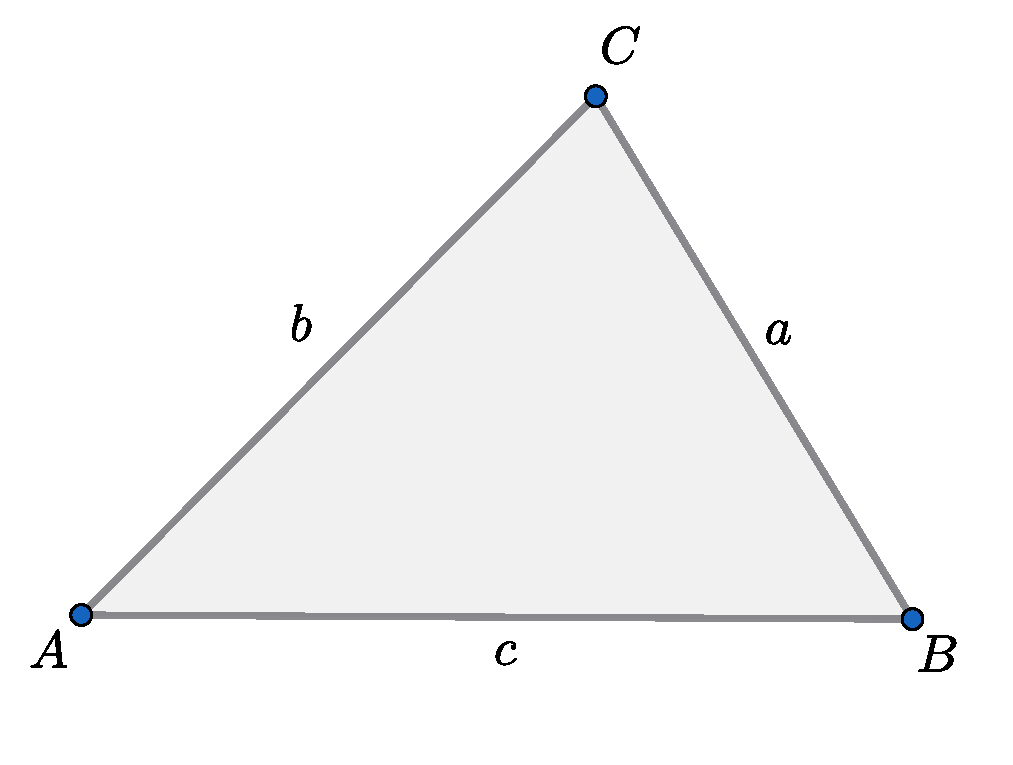
\includegraphics[scale=0.4]{25}
    	\caption{}
       \label{Figure25}
\end{figure} 
\begin{theorembox}[กฏของไซน์]
กำหนดให้ $\triangle ABC$ ถูกล้อมรอบด้วยวงกลมรัศมี $R$ แต่มีความยาวแต่ละด้านซึ่งแสดงดังรูปที่~\ref{Figure26} เราจะได้ความสัมพันธ์ว่า
\[\frac{a}{\sin(A)}=\frac{b}{\sin(B)}=\frac{c}{\sin(C)}=2R\]
\end{theorembox}
 \begin{figure}[H]	 
	\centering
	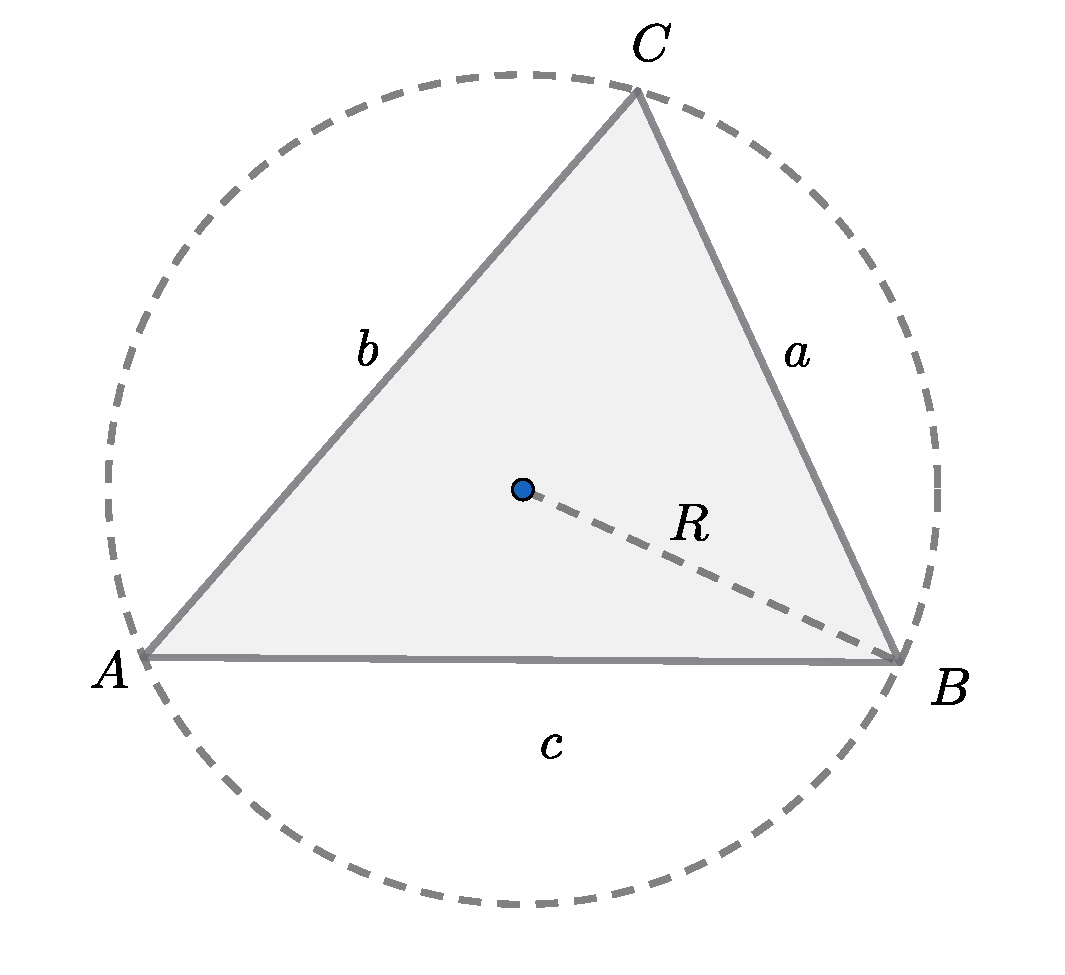
\includegraphics[scale=0.4]{26}
    	\caption{}
       \label{Figure26}
\end{figure} 

\newpage
\begin{examplebox}[NETSAT คณิตศาสตร์ สิงหาคม 2568]  
กำหนดให้ $\triangle ABC$ มี $AB=3$ หน่วย $AC=3$ หน่วย และ $\angle A =120^{\circ}$ จงหาความยาวด้าน $BC$
\begin{enumerate}
\item $3\sqrt{3}$
\item $3\sqrt{5}$
\item $3\sqrt{7}$
\item $9$
\end{enumerate}
\end{examplebox}

\begin{examplebox}[NETSAT คณิตศาสตร์ 2566]
จากรูปที่~\ref{Figure27} จงหาขนาดของมุม $B$
\begin{enumerate}
\item $30^{\circ}$
\item $45^{\circ}$
\item $60^{\circ}$
\item $75^{\circ}$
\end{enumerate}
\end{examplebox} 
\begin{figure}[H]	 
	\centering
	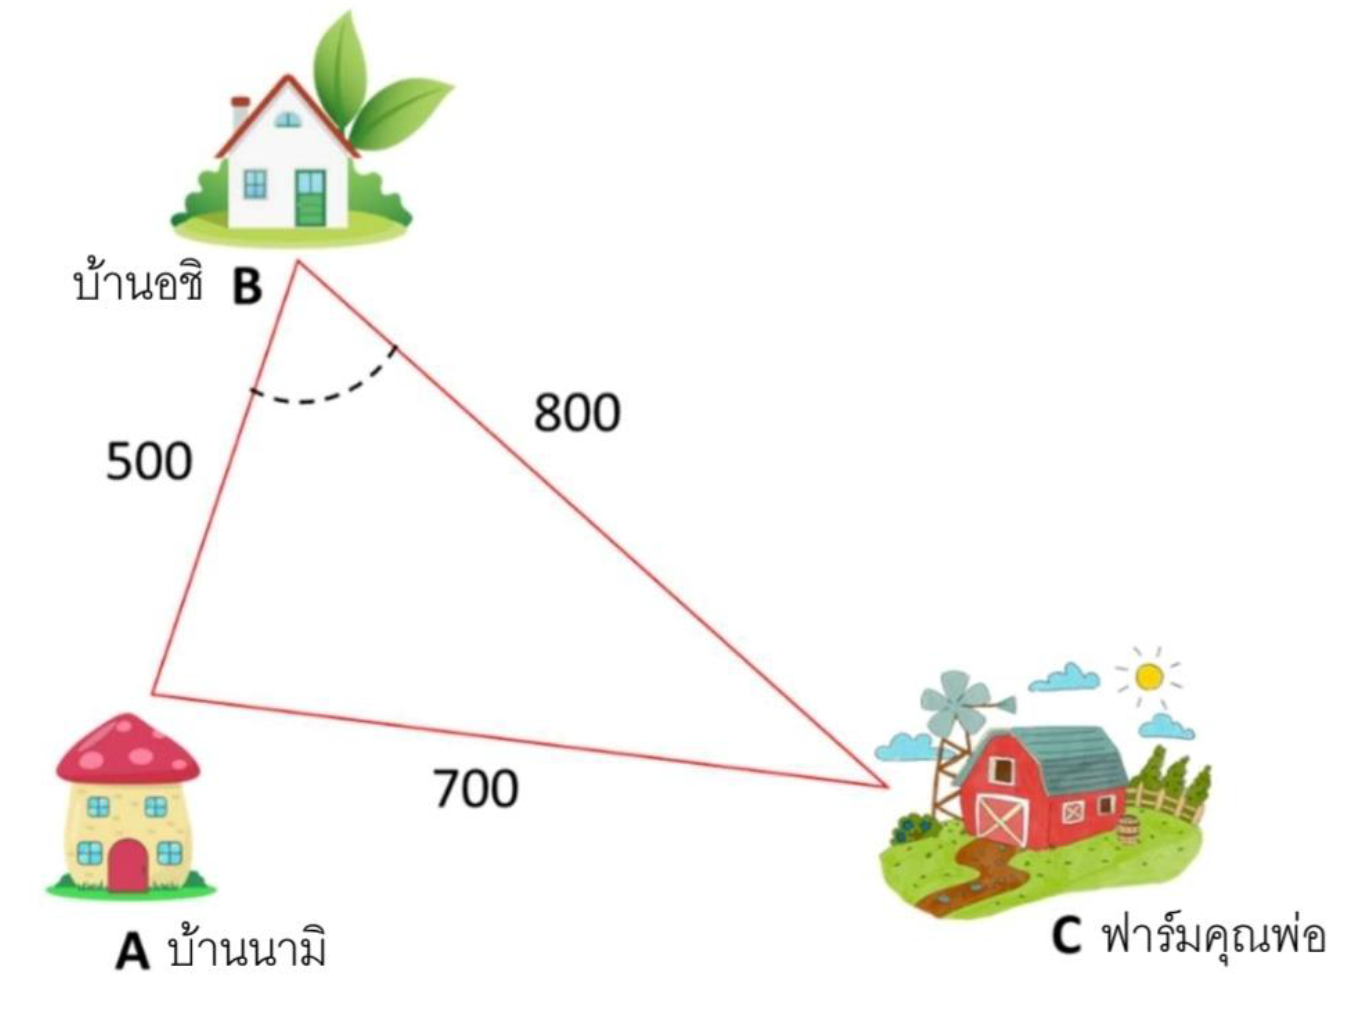
\includegraphics[scale=0.6]{27}
    	\caption{}
       \label{Figure27}
\end{figure} 

\newpage
\begin{examplebox}[NETSAT คณิตศาสตร์ 2566]
รูปที่~\ref{Figure28} แสดงภาพมุมสูงของม้าหมุนในสวน แห่งหนึ่ง โดยมีที่นั่งอยู่บนเส้นรอบวงสองวง และ หมุนรอบจุดศูนย์กลาง $O$ โดยมีรัศมีของวงกลมด้าน นอกเท่ากับ $10$ เมตร รัศมีของวงกลมด้านในเท่ากับ $6$ เมตร
กำหนดให้ที่นั่ง $A$ และ $B$ อยู่ข้างกันบนเส้นรอบวงด้าน นอก และด้านในตามลำดับ โดยไม่คำนึงขนาดของที่นั่ง เมื่อที่นั่ง $A$ และ $B$ เริ่มขยับไปพร้อมๆ กัน รูปที่ 2 แสดงให้เห็นตำแหน่ง $A$ และ $B$ หลังผ่านไป $2-3$ นาที หลังจากเริ่มหมุน ถ้า $\angle AOB=\theta$ และ $\cos(\theta)=\dfrac{11}{24}$ จงหาระยะทางจาก $A$ มา $B$
\begin{enumerate}
\item $7$
\item $9$
\item $11$
\item $13$
\end{enumerate}
\end{examplebox} 
\begin{figure}[H]	 
	\centering
	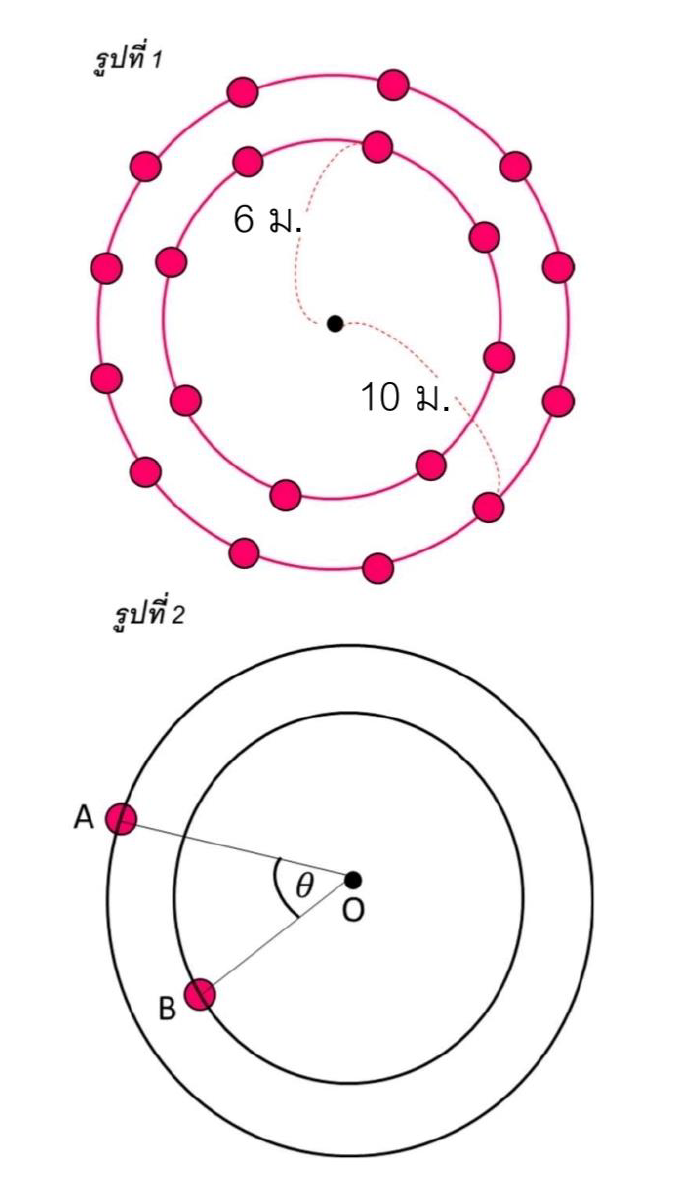
\includegraphics[scale=0.7]{28}
    	\caption{}
       \label{Figure28}
\end{figure}